\documentclass[conference]{IEEEtran}
\IEEEoverridecommandlockouts
% The preceding line is only needed to identify funding in the first footnote. If that is unneeded, please comment it out.
\usepackage{cite}
\usepackage{amsmath,amssymb,amsfonts}
\usepackage{algorithmic}
\usepackage{graphicx}
\usepackage{textcomp}
\usepackage{xcolor}
\usepackage[brazilian]{babel}
\usepackage[utf8]{inputenc}
\usepackage[T1]{fontenc}
\usepackage{listings}
\usepackage{color}
\usepackage{float}
\usepackage{multirow}
\usepackage{hyperref}

\definecolor{dkgreen}{rgb}{0,0.6,0}
\definecolor{gray}{rgb}{0.5,0.5,0.5}
\definecolor{mauve}{rgb}{0.58,0,0.82}

\lstset{frame=tb,
  language=Java,
  aboveskip=3mm,
  belowskip=3mm,
  showstringspaces=false,
  columns=flexible,
  basicstyle={\small\ttfamily},
  numbers=none,
  numberstyle=\tiny\color{gray},
  keywordstyle=\color{blue},
  commentstyle=\color{dkgreen},
  stringstyle=\color{mauve},
  breaklines=true,
  breakatwhitespace=true,
  tabsize=3
}
\lstset{language=Python}
\def\BibTeX{{\rm B\kern-.05em{\sc i\kern-.025em b}\kern-.08em
    T\kern-.1667em\lower.7ex\hbox{E}\kern-.125emX}}
\begin{document}

\title{Relatório do Laboratório 7: \\ Redes Neurais\\
}

\author{\IEEEauthorblockN{Isabelle Ferreira de Oliveira}
\IEEEauthorblockA{\textit{CT-213 - Engenharia da Computação 2020} \\
\textit{Instituto Tecnológico de Aeronáutica (ITA)}\\
São José dos Campos, Brasil \\
isabelle.ferreira3000@gmail.com}
}

\maketitle

\begin{abstract}
Esse relatório documenta a implementação de uma rede neural de duas camadas para realizar a segmentação de cores para o futebol de robôs. Para isso, foi necessário configurar essa rede neural para realizar classificação multi-classe, implementando os algoritmos de Forward Propagation (inferência) e Back Propagation (treinamento) para essa rede.
\end{abstract}

\begin{IEEEkeywords}
Redes neurais, segmentação de cores, \textit{Forward Propagation}, \textit{Back Propagation}
\end{IEEEkeywords}

\section{Introdução}
Redes neurais são sistemas de computação que podem reconhecer padrões escondidos, agrupar dados e classificá-los, além de, com o tempo, aprender e melhorar continuamente \cite{sas}.

Uma rede neural é formada por camadas de neurônios artificiais (baseado no sistema nervoso humano e neurônios naturais), e eles são os responsáveis por realizar as contas que levam de uma entrada a uma saída esperada (para o caso de aprendizado supervisionado). A Figura \ref{rede_neural} apresenta um exemplo de rede neural com duas camadas (a camada de entrada geralmente não é considerada nesse tipo de contagem). É possível notar no exemplo que a camada 1 tem 3 neurônios e a camada 2 tem 1 neurônio. 

\begin{figure}[htbp]
\centering
\centerline{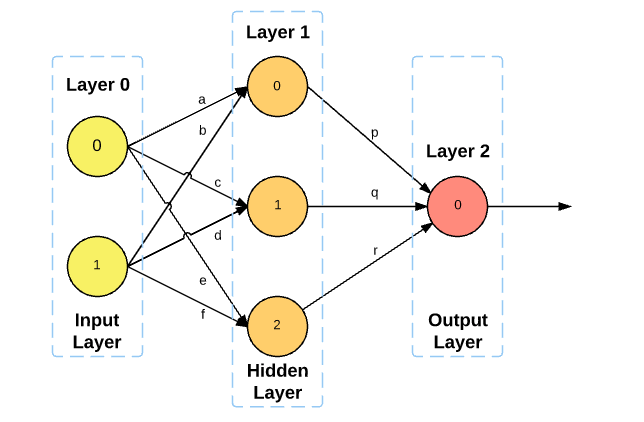
\includegraphics[scale=0.4]{imagens/rede_neural.png}}
\caption{Exemplo de rede neural, com duas camadas (1 camada de entrada, 1 camada escondida e 1 camada de saída), como a trabalhada nesse laboratório. Essa imagem de exemplo foi apresentada no site \cite{neural-net-np}}.
\label{rede_neural}
\end{figure}

Agora analizando um neurônio em particular, como o apresentado na Figura \ref{neuronio}, a conta realizada para o aprendizado é que se encontra no interior do círculo, ou seja: $g\left ( \sum w_j x_j + b \right ) = y$, no qual $w$ são os pesos; $b$, os bias; $x$, as entradas; e $g$, a função de ativação. O objetivo do treinamento é ajustar $w$ e $b$ para aproximar alguma função y(x) de acordo com os valores fornecidos como \textit{outputs} esperados.

\begin{figure}[htbp]
\centering
\centerline{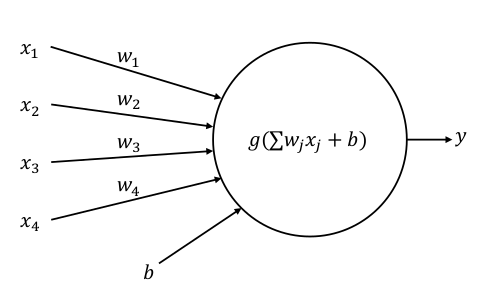
\includegraphics[scale=0.4]{imagens/neuronio.png}}
\caption{Exemplo de neurônio. Essa imagem de exemplo foi apresentada no roteiro \cite{roteiro}}.
\label{neuronio}
\end{figure}

O processo de inferência é realizado por meio do cálculo da equação apresentada no círculo do neurônio da Figura \ref{neuronio}, em um algoritmo chamado \textit{Forward Propagation}. Já o processo de aprendizado é realizado pelo algoritmo de \textit{Back Propagation}, que calcula os pesos e \textit{biases} a partir das saídas esperadas e das decidas de gradientes calculados para esses pesos e \textit{bias}. Já esses gradientes são calculados por meio das saídas esperadas, as entradas iniciais e os resultados intermediários calculados por meio do \textit{Forward Propagation}. 

Os pseudo-códigos geral dos algortimos \textit{Forward Propagation}, \textit{Back Propagation} e o cálculo das decidas de gradientes para pesos e \textit{biases} podem ser visto a seguir. Em seguida, será apresentado como esses algoritmos foram implementados no contexto do laboratório.

\begin{lstlisting}
# Forward Propagation
def forward_propagation(input):
	z[1] = weights[1]input + biases[1]
	a[1] = g[1](z[1])
	z[2] = weights[2]a[1] + biases[2]
	a[2] = g[2](z[2])
	return z, a
\end{lstlisting}

\begin{lstlisting}
# Gradients' Computation
def compute_gradient_back_propagation(inputs, expected_outputs):
	for i in range(len(inputs)):
		input = inputs[i]
		expected_output = expected_outputs[i]
		
		z, a = forward_propagation(input)

		dz[2] = a[2] - expected_output
		weights_gradient[2] += dz[2] a[1].T
		biases_gradient[2] += dz[2]

		dz[1] = weights[2].T dz[2] * derivate(g[1](z[1]))
		weights_gradient[1] += dz[1] input.T
		biases_gradient[1] += dz[1]

	return weights_gradient, biases_gradient
\end{lstlisting}

\begin{lstlisting}
# Back Propagation
def back_propagation(inputs, expected_outputs):
	weights_gradient, biases_gradient = compute_gradient_back_propagation(inputs, expected_outputs)

	weights[1] -= alpha * weights_gradient[1]
	biases[1] -= alpha * biases_gradient[1]
	weights[2] -= alpha * weights_gradient[2]
	biases[2] -= alpha * biases_gradient[2]
\end{lstlisting}

No pseudocódigo acima, \textit{J} é a função para medir a qualidade das soluções candidatas; \textit{m0} e \textit{C0} são a média e a matriz de covariância iniciais da população que será gerada, respectivamente; \textit{m} e \textit{C} são, de forma análoga, a média e a matriz de covariância atuais da população que será gerada, respectivamente; e \textit{mu} é o tamanho da população considerada como "melhores soluções até então".

\section{Implementação do algoritmo}
Para a implementação da rede neural, era necessário preencher a função \textit{forward\underline{\space}propagation()}, \textit{compute\underline{\space}gradient\underline{\space}back\underline{\space}propagation()} e \textit{back\underline{\space}propagation()} da classe \textit{NeuralNetwork}. Essas funções a se completar estavam no código base fornecido \cite{roteiro}.  

Recebendo os valores de \textit{input}, a função \textit{forward\underline{\space}propagation()} foi implementada conforme apresentado no pseudo-código da Introdução, com o detalhe que a função de ativação $g$ de todos os neurônios utilizada foi a \textit{sigmoid}. Além disso, tanto a função \textit{sigmoid} quanto sua derivada já eram fornecidos pelo código base. 

Já na implementação de \textit{back\underline{\space}propagation()}, também foi implementado conforme o sugerido no pseudo-código da Introdução, ou seja, atualizando os valores de pesos e \textit{biases} subtraindo de seu valor um fator de aprendizado \textit{alpha} vezes os gradientes de pesos e \textit{biases}, respectivamente. Esses valores de gradientes são aqueles calculados em \textit{compute\underline{\space}gradient\underline{\space}back\underline{\space}propagation()}, supondo que essa função já foi corretamente implementado. Foi utilizado para \textit{alpha} o mesmo que o sugerido pelo código base. 

Finalmente, para implementar a função \textit{compute\underline{\space}gradient\underline{\space}back\underline{\space}propagation()}, também foi feito de forma bastante semelhante ao apresentado na Introdução, com o detalhe de usar \textit{numpy.multiply} para multiplicar termo a termo os vetores referentes aos pesos e a derivada da função de ativação.

Para testar o funcionamento dessas implementações, foi inicialmente alterado o valor da variável \textit{classification\underline{\space}function} (entre "sum\underline{\space}gt\underline{\space}zero" no arquivo \textit{test\underline{\space}neural\underline{\space}network.py} do código base, gerando imagens dos resultados da classificação de cada \textit{dataset} para cada uma dessas funções (função "soma maior que zero" e função "xor") usando rede neural.

Já tendo ciência da correta implementação dos algoritmos de aprendizado, foi feito por fim um teste da segmentação de cores, executando o código do arquivo \textit{test\underline{\space}color\underline{\space}segmentation.py}, conforme indicado no roteiro \cite{roteiro}. Os gráficos de resultados tanto dessa segmentação de cores, quanto das funções anteriores, foram apresentados nas Figuras \ref{sum_gt_zero/cost_function_convergence} a \ref{color_segmentation/segmented_image}.

\section{Resultados e Conclusões}

\subsection{Teste das Estratégias Evolutivas}

A otimização para testar a implementação foi executada para as quatro funções evolutivas já citadas na seção anterior, cuja equação matemática se encontra no roteiro do laboratório \cite{b1}. Os resultados dessas execuções foram satisfatórios e saíram conforme o esperado, comprovando o correto funcionamento da implementação e a validade da utilização das estratégias evolutivos na otimização de funções. Esses resultados foram apresentados nas Figuras de \ref{translated_sphere/ses} a \ref{rastrigin/cmaes}.

Vale reparar que os resultados de ambas implementações foram bastante equivalentes, com exceção do caso da função Rastrigin, no qual cada algoritmo convergiu em míminos locais diferentes.

\begin{figure}[htbp]
\centering
\centerline{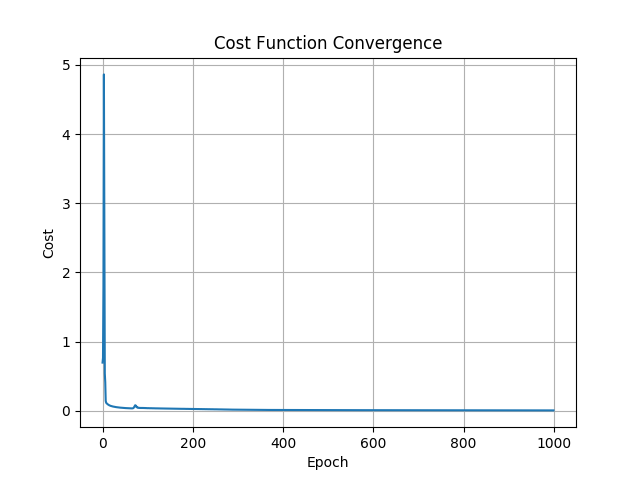
\includegraphics[scale=0.5]{imagens/sum_gt_zero/cost_function_convergence.png}}
\caption{Otimização da função de Esfera Transladada usando a estratégia evolutiva SES. O resultado encontrado é o ponto vermelho.}
\label{sum_gt_zero/cost_function_convergence}
\end{figure}

\begin{figure}[htbp]
\centering
\centerline{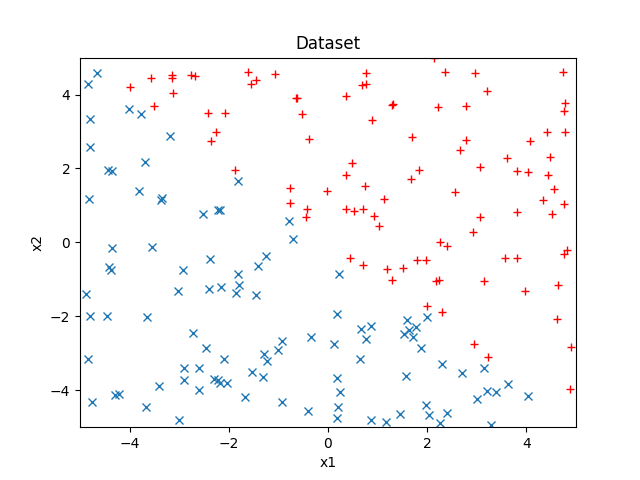
\includegraphics[scale=0.5]{imagens/sum_gt_zero/dataset.png}}
\caption{Otimização da função de Esfera Transladada usando a estratégia evolutiva CMA-ES. O resultado encontrado é o ponto vermelho.}
\label{sum_gt_zero/dataset}
\end{figure}

\begin{figure}[htbp]
\centering
\centerline{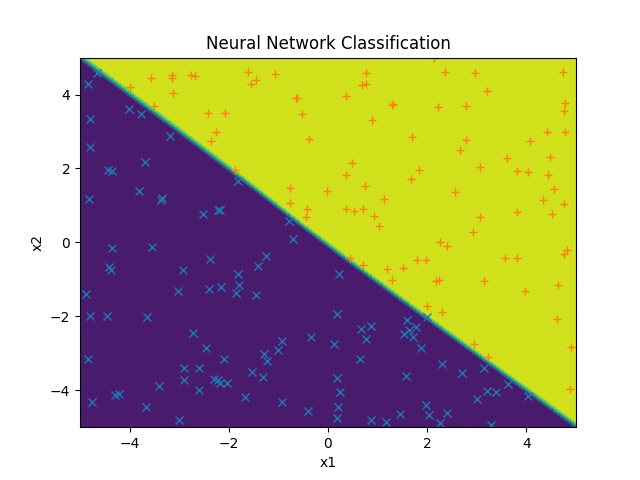
\includegraphics[scale=0.5]{imagens/sum_gt_zero/neural_net_classification.png}}
\caption{Otimização da função de Ackley usando a estratégia evolutiva SES. O resultado encontrado é o ponto vermelho.}
\label{sum_gt_zero/neural_net_classification}
\end{figure} 

\begin{figure}[htbp]
\centering
\centerline{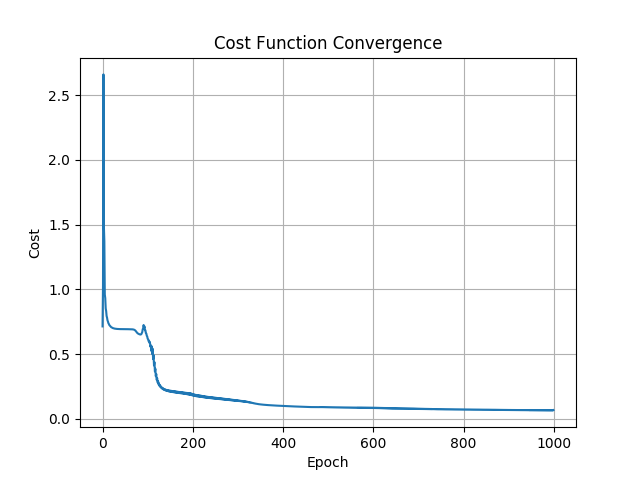
\includegraphics[scale=0.5]{imagens/xor/cost_function_convergence.png}}
\caption{Otimização da função de Esfera Transladada usando a estratégia evolutiva SES. O resultado encontrado é o ponto vermelho.}
\label{xor/cost_function_convergence}
\end{figure}

\begin{figure}[htbp]
\centering
\centerline{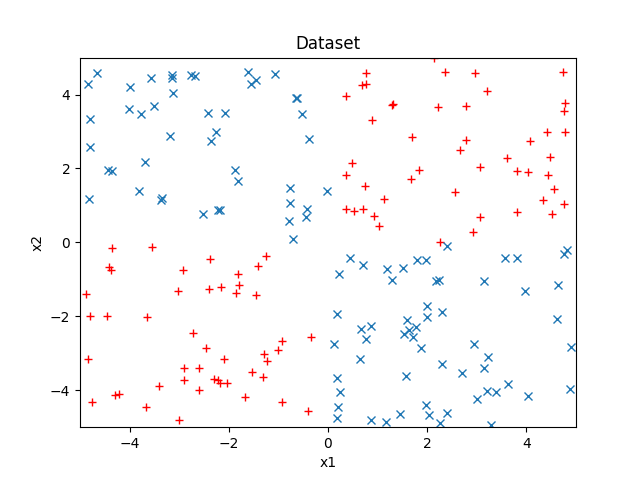
\includegraphics[scale=0.5]{imagens/xor/dataset.png}}
\caption{Otimização da função de Esfera Transladada usando a estratégia evolutiva CMA-ES. O resultado encontrado é o ponto vermelho.}
\label{xor/dataset}
\end{figure}

\begin{figure}[htbp]
\centering
\centerline{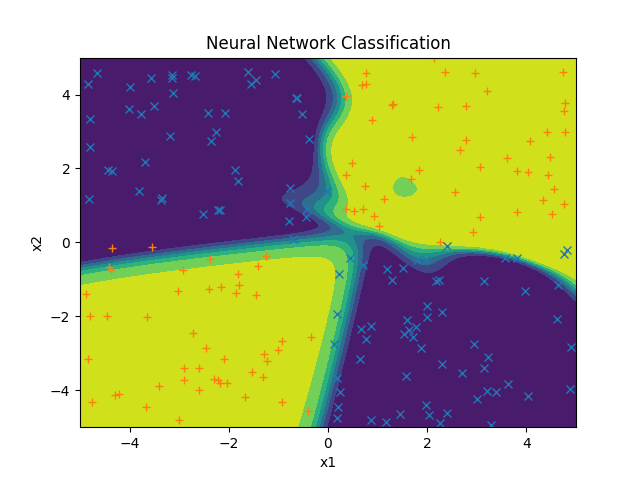
\includegraphics[scale=0.5]{imagens/xor/neural_net_classification.png}}
\caption{Otimização da função de Ackley usando a estratégia evolutiva SES. O resultado encontrado é o ponto vermelho.}
\label{xor/neural_net_classification}
\end{figure} 

\begin{figure}[htbp]
\centering
\centerline{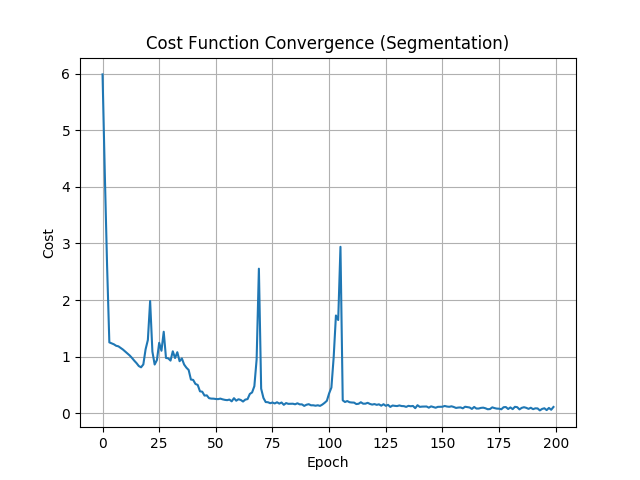
\includegraphics[scale=0.5]{imagens/color_segmentation/cost_function_convergence_segmentation.png}}
\caption{Otimização da função de Esfera Transladada usando a estratégia evolutiva SES. O resultado encontrado é o ponto vermelho.}
\label{color_segmentation/cost_function_convergence_segmentation}
\end{figure}

\begin{figure}[htbp]
\centering
\centerline{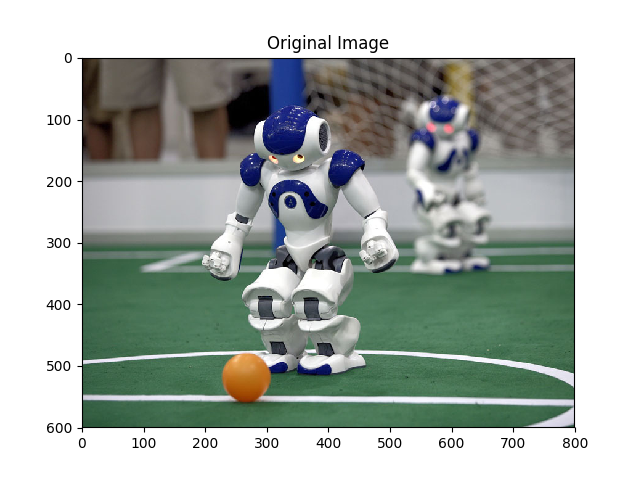
\includegraphics[scale=0.5]{imagens/color_segmentation/original_image.png}}
\caption{Otimização da função de Esfera Transladada usando a estratégia evolutiva CMA-ES. O resultado encontrado é o ponto vermelho.}
\label{color_segmentation/original_image}
\end{figure}

\begin{figure}[htbp]
\centering
\centerline{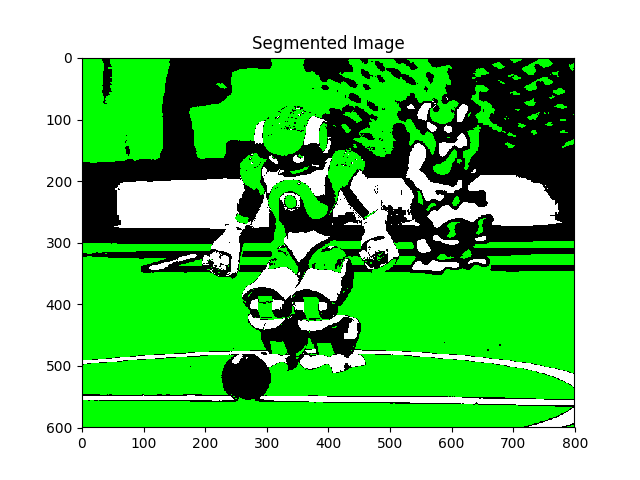
\includegraphics[scale=0.5]{imagens/color_segmentation/segmented_image.png}}
\caption{Otimização da função de Ackley usando a estratégia evolutiva SES. O resultado encontrado é o ponto vermelho.}
\label{color_segmentation/segmented_image}
\end{figure} 

\subsection{Benchmark das Estratégias Evolutivas}

A otimização para realizar o \textit{benchmark} do desempenho de cada um dos métodos evolutivos estudados (SES e CMA-ES) para diferentes funções e parâmetros foi executada para as quatro funções evolutivas já citadas. Os resultados dessas execuções demonstraram comportamentos coerentes e foram apresentados nas Figuras de \ref{translated_sphere/ses} a \ref{rastrigin/cmaes}.

É possível salientar que, embora sempre tenha havido convergências após um número significativo de iterações, nem todas as convergências chegaram a mínimos locais, como por exemplo para a função da Esfera Transaladada, que só possui um mínimo local (que também é global), mas cada situação testada chegou a valores diferentes de \textit{fitness}.

Além disso, notou-se que, para estratégias evolutivas mais simples, é necessário um número cada vez maior de elementos na população para que os resultados se tornem cada vez mais otimizados. Já para o algoritmo CMA-ES precisou de cerca de 1/4 de população para alcançar resultados similares aos do SES. Isso aconteceu para todos os casos com exceção à função Schaffer Nº 2, que estratégias mais simples e com menores populações se saíram melhor em desempenho do que CMA-ES.

Tendo em vista o que foi apresentado, pode-se notar, por fim, que esses algoritmos realmente se demonstraram eficazes em encontrar parâmetros otimizados para uma determinada função.

\begin{thebibliography}{00}
\bibitem{roteiro} M. Maximo, ``Roteiro: Laboratório 5 - Estratégias Evolutivas''. Instituto Tecnológico de Aeronáutica, Departamento de Computação. CT-213, 2019.

\bibitem{neural-net-np} Towards Data Science, "Neural Net from scratch". Acessado em https://towardsdatascience.com/neural-net-from-scratch-using-numpy-71a31f6e3675.

\bibitem{sas} SAS, "Redes Neurais: O que são e qual a sua importância?". Acessado em https://www.sas.com/pt\underline{\space}br/insights/analytics/neural-networks.html.

\end{thebibliography}

\end{document}
